%\section{Derived classes}\index{derived class, object oriented programming}

As we have seen, the \texttt{OpenNN} neural network is composed by a multilayer perceptron plus some other kinds of layers. 
In this section we study the software model of the \lstinline"NeuralNetwork" class. 


\subsection*{Classes}

The characterization in classes of the concepts studied in the previous section is as follows:

\begin{description}

\item[Perceptron] The class which represents the concept of perceptron neuron model is called \lstinline"Perceptron".

\item[PerceptronLayer] The class representing a layer of perceptrons is called \lstinline"PerceptronLayer".

\item[MultilayerPerceptron] The class which represents a feed-forward architecture of perceptron layers is called \lstinline"MultilayerPerceptron".

\item[Scaling layer] The class which represents a layer for scaling variables is called \lstinline"ScalingLayer".

\item[Unscaling layer] The class which represents an unscaling layer is called \lstinline"UnscalingLayer".
 
\item[Bounding layer] The class representing a layer of bounding neurons is called \lstinline"BoundingLayer".

\item[Conditions layer] The class wich applies input-output conditions is called \lstinline"ConditionsLayer".

\item[Independent parameters] A class containing parameters not belonging to the multilayer perceptron is called \lstinline"IndependentParameters".

\item[Neural network] The class which aggregates all the different neural network concepts is called \lstinline"NeuralNetwork".

\end{description}

\subsection*{Associations}

The appropriate associations between all the neural networks classes in the system are next identified to be included
to the association diagram:

\begin{description}

\item[Perceptron layer - perceptron] A layer of perceptrons is composed of perceptrons.

\item[Multilayer perceptron - perceptron layer] A multilayer perceptron is composed of layers of perceptrons.

\item[Neural network - Multilayer perceptron] A neural network very probably contains a multilayer perceptron.

\item[Neural network - Scaling layer] A multilayer perceptron usually contains a scaling layer. 

\item[Neural network - Unscaling layer] A multilayer perceptron usually contains an unscaling layer. 

\item[Neural network - Bounding layer] A multilayer perceptron sometimes contains a bounding layer.

\item[Neural network - Probabilistic layer] A multilayer perceptron sometimes contains a probabilistic layer.

\item[Neural network - Conditions layer] A multilayer perceptron might contain a conditions layer.

\item[Neural network - Independent parameters] A multilayer percetpron might contain a set of independent parameters.    

\end{description}

Figure \ref{NeuralNetworkAssociationDiagram} depicts an association diagram
for the neural network class. 

\begin{figure}[h!]
\begin{center}
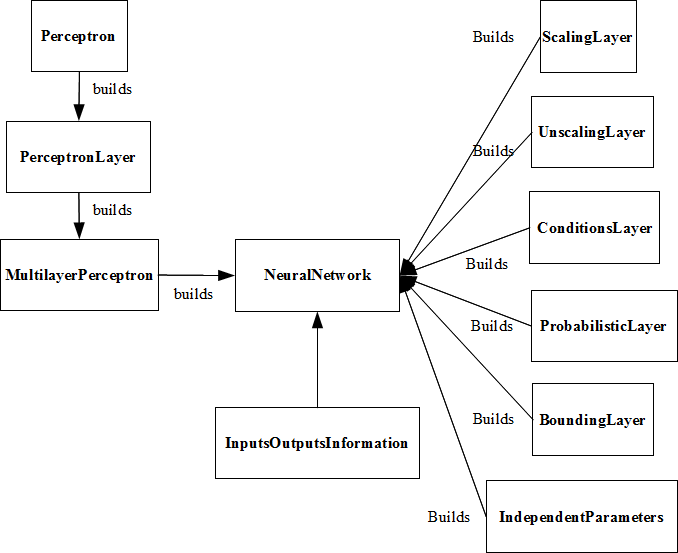
\includegraphics[width=1.1\textwidth]{neural_network/association_diagram}
\caption{Association diagram for the \lstinline'NeuralNetwork' class.}\label{NeuralNetworkAssociationDiagram}
\end{center}
\end{figure}

\subsection*{Derived classes}

The next task is then to establish which classes are abstract and
to derive the necessary concrete classes to be added to the
system. 

The neural network class in \texttt{OpenNN} will be intensively used by any application. 
Therefore, for performance reasons, all the composing classes have been designed to be concrete. 

Let us then examine the classes we have so far:

\begin{description}

\item[Perceptron] The class \lstinline"Perceptron" is concrete,
and can implement different activation functions. 

\item[Perceptron layer] The class \lstinline"PerceptronLayer" is also concrete,
since it is defined as a vector of perceptrons.

\item[Multilayer perceptron] The class \lstinline"MultilayerPerceptron" is a concrete class and is
itself suitable for instantiation. This class is implemented as a vector of layers of perceptrons. 

\item[Scaling layer] The class \lstinline"ScalingLayer" is concrete, and implements the minimum-maximum and mean-standard deviation scaling methods.

\item[Unscaling layer] The class \lstinline"UnscalingLayer" is also concrete, and implements the minimum-maximum and mean-standard deviation unscaling methods.

\item[Bounding layer] The class \lstinline"BoundingLayer" is concrete. It sets to their bound values those inputs which are below or above them. 

\item[Probabilistic layer] The class \lstinline"ProbabilisticLayer" is concrete, and implements the competitive and softmax methods.

\item[Conditions layer] The class \lstinline"ConditionsLayer" has also been designed to be concrete. It implements methods to hold one or two condions. For more difficult situations, further classes must be derived. 

\item[Inputs-outputs information] The class \lstinline"InputsOutputsInformation" is concrete. It mainly stores a few strings with the names, units and descriptions of the neural network variables. 

\item[Independent parameters] The class \lstinline"IndependentParameters" is concrete. It contains other adjustable parameters 
than those belonging to the multilayer perceptron. 

\end{description}

\subsection*{Attributes and operations}

An attribute is a named value or relationship that exists for all
or some instances of a class. An operation is a procedure
associated with a class \cite{Stroustrup2000}. 

In UML class
diagrams, classes are depicted as boxes with three sections: the
top one indicates the name of the class, the one in the middle
lists the attributes of the class, and the bottom one lists the
operations \cite{Rumbaugh1999}.


\begin{description}

\item[Perceptron] A perceptron neuron model has the following attributes:

\begin{itemize}
\item[-] A bias.
\item[-] A set of synaptic weights.
\item[-] The activation function.
\end{itemize}

It performs the following main operations:

\begin{itemize}
\item[-] Calculate the neuron output for a given input.
\item[-] Calculate the derivatives of the output with respect to the inputs.
\end{itemize}


\item[Perceptron layer] The perceptron layer has the following members:

\begin{itemize}
\item[-] A set of perceptrons.
\end{itemize}
 
It performs the following methods:

\begin{itemize}
\item[-] Calculate the layer output for a given input.
\item[-] Calculate the derivatives of the outputs with respect to the inputs.
\end{itemize}

\item[Multilayer perceptron] A multilayer perceptron has the following attributes:

\begin{itemize}
\item[-] A set of layers of perceptrons.
\end{itemize}

It performs the following main operations:

\begin{itemize}
\item[-] Calculate the output for a given input.
\item[-] Calculate the Jacobian for a given input.
\item[-] Calculate the Hessian form for a given input.
\end{itemize}

\item[Scaling layer] The scaling layer has the following members:

\begin{itemize}
\item[-] The main statistics of the variables.
\item[-] The scaling method.
\end{itemize}

It implements the following main members:

\begin{itemize}
\item[-] Calculate the scaled variables for unscaled variables.
\item[-] Calculate the derivatives of the scaling function.
\end{itemize}

\item[Unscaling layer] The unscaling layer is similar to the scaling layer, 
with the following members:

\begin{itemize}
\item[-] The main statistics of the variables.
\item[-] The unscaling method.
\end{itemize}

It implements the following main members:

\begin{itemize}
\item[-] Calculate the unscaled variables for scaled variables.
\item[-] Calculate the derivatives of the unscaling function.
\end{itemize}

\item[Bounding layer] The bounding layer contains the following attributes:

\begin{itemize}
\item[-] The lower and upper bounds of the variables.
\end{itemize}

It performs the following main operations:

\begin{itemize}
\item[-] Calculate bounded variables for unbounded ones.
\item[-] Calculate the derivatives of the bounding function.
\end{itemize}

\item[Probabilistic layer] The probabilist layer contains:

\begin{itemize}
\item[-] The probabilistic method.
\end{itemize}

It computes the following functions:

\begin{itemize}
\item[-] Calculate probabilistic variables for non-probabilistic ones.
\item[-] Calculate also the derivatives.
\end{itemize}

\item[Conditions layer] The conditions layer contains the following:

\begin{itemize}
\item[-] The conditions values.
\item[-] The conditions method.
\end{itemize}

   
It performs the following:

\begin{itemize}
\item[-] Calculate outputs holding some conditions. 
\item[-] Calculate also the derivatives of that conditioned outputs.
\end{itemize}

\item[Inputs-outputs information] This class stores the following data:

\begin{itemize}
\item[-] The names, units and descriptions of the input and output variables.
\end{itemize}

It performs the following:

\begin{itemize}
\item[-] Write default names for the inputs and the outputs. 
\end{itemize}

\item[Independent parameters] The class representing independent parameters contains the following main members:

\begin{itemize}
\item[-] A set of parameters.
\item[-] Information and statistics on the parameters.
\item[-] Scaling/Unscaling and bounding methods. 
\end{itemize}

The independent parameters class can perform the follwoing operations:

\begin{itemize}
\item[-] Scale and unscale the parameters.
\item[-] Bounding the parameters. 
\end{itemize}

\end{description}



